\section{Sampling random points within \emph{d}-dimensional domains by hit and
miss}
I skipped the integration on the rectangle, solving only the disk case.  The
source code is in \texttt{A01b\_disk\_hit\_miss.c}; I implemented the main part
of the algorithm like this:
\lstinputlisting[
    firstline=32, lastline=46, language=C
]{../src/A01b_disk_hit_miss.c}
The error as a function of the number of throws is shown in \figref{fig:A01b}.
It is comfortably under \qty{1}{\percent} with around \numrange{25000}{30000}
iterations.

\begin{figure}
    \centering
    \includesvg[inkscapelatex=false]{img/A01b.svg}
    \caption{error in the Monte Carlo estimation of the area of a unit
        disk, as a function of the number of \textquote{throws}.}
    \label{fig:A01b}
\end{figure}

\section{Sampling random numbers from a given distribution}
The idea is to sample from the probability distribution $\rho_n(x) = c x^n$ in
$[0, 1]$.  First, using the normalization condition we can find out what $c$
should be:
\begin{equation}
    1 = \int_{0}^{1} cx^n \, dx = \frac{c}{n + 1} \implies c = n + 1.
\end{equation}
Then, we find the expression of the associated cumulative density function:
\begin{equation}
    F_n(x) = (n + 1) \int_{0}^{x} y^n \, dy = x^{n + 1},
\end{equation}
and invert it:
\begin{equation}
    u = x^{n + 1} \implies x = u^{1 / (n + 1)}.
\end{equation}

So, inside the code \texttt{A02a\_inversion\_method.c} I sample a random
\texttt{double} from a uniform distribution between $0$ and $1$ using
\texttt{drand48()}, and I raise it to the power of $1 / (n + 1)$ to get $x$:
\lstinputlisting[
    firstline=25, lastline=27, language=C
]{../src/A02a_inversion_method.c}
A histogram of \num{100000} points sampled from $\rho$ with $n = 3$ is displayed
in \figref{fig:A02a_3}.

\begin{figure}
    \centering
    \includesvg[inkscapelatex=false]{img/A02a_3.svg}
    \caption{histogram of \num{100000} points sampled from the probability
        distribution $4 x^3$ in $[0, 1]$.}
    \label{fig:A02a_3}
\end{figure}

Inside \texttt{A02b\_inversion\_method.c} I modified the code to sample from
$\rho_2(x) = cx^2$ in $[0, 2]$. This time $c$ is different, of course:

\begin{equation}
    1 = \int_{0}^{2} cx^2 \, dx = \frac{8}{3}c \implies c = \frac{3}{8}.
\end{equation}
The cumulative is then
\begin{equation}
    F_2(x) = \frac{3}{8} \int_{0}^{x} y^2 \, dy = \frac{x^3}{8} \implies x = 2
    u^{1/3}.
\end{equation}
Once again, you can see the comparison between a \num{100000}-points histogram
and the theoretical curve in \figref{fig:A02b}.

\begin{figure}
    \centering
    \includesvg[inkscapelatex=false]{img/A02b.svg}
    \caption{histogram of \num{100000} points sampled from the probability
        distribution $3x^2/8$ in $[0, 2]$.}
    \label{fig:A02b}
\end{figure}

\section{Sampling via transformation of coordinates}
If we want to sample points uniformly distributed over the unit disk, we cannot
simply generate $r \sim \unif{0}{1}$ and $\theta \sim \unif{0}{2\pi}$. The
result of doing that is shown in \figref{subfig:A03aa}, with the corresponding
source code in \texttt{A03aa\_disk\_naive.c}. While the angular distribution
poses no problem, there is an undesired higher density of points close to the
centre of the disk.

\begin{figure}
    \centering
    \begin{minipage}[t]{0.5\linewidth}
        \centering
        \includesvg[inkscapelatex=false]{img/A03aa.svg}
        \subcaption{}
        \label{subfig:A03aa}
    \end{minipage}\hfill%
    \begin{minipage}[t]{0.5\linewidth} 
        \centering
        \includesvg[inkscapelatex=false]{img/A03ab.svg}    
        \subcaption{}
        \label{subfig:A03ab}
    \end{minipage}
    \caption{\num{10000} points sampled on the unit disk with the wrong
        coordinate transformation (a) and with the correct one (b).}
    \label{fig:A03a}
\end{figure}

The reason for this becomes clear when you consider the number of points falling
inside a ring of given thickness $\delta r$. Consider a ring with inner radius
$r_1$ and outer radius $r_1 + \delta r$, with $\delta r \ll r_1$, and another
with radii $r_2$, $r_2 + \delta r$.  Despite the ratio of their areas being $r_2
/ r_1$, the fraction of points within each ring remains the same. Thus, the
number of points falling at a distance $r$ should instead be proportional to $r$
\begin{equation}
    \rho_{r}(r) = 2r,
\end{equation}
with the $2$ in front to ensure normalization over $[0, 1]$. By computing the
cumulative and inverting we get 
\begin{equation}
    F_r(r) = 2 \int_{0}^{x} x \, dx = x^{2} \implies u = r^{2} \implies r =
    \sqrt{u}.
\end{equation}

So, I modified the code in \texttt{A03ab\_disk\_correct.c} to sample like this:
\lstinputlisting[
    firstline=25, lastline=32, language=C
]{../src/A03ab_disk_correct.c}
The result is the correctly uniform sampling in \figref{subfig:A03ab}.

As regards the Box–Muller transform, I started from the factorization of
$\rho_{x, y}(x, y)$:
\begin{equation}
    \rho_{x, y}(x, y) = \frac{1}{2\pi} \exp\left(-\frac{x^{2} + y^{2}}{2}\right)
        = \rho_x(x) \rho_y(y), \quad \text{with }
        \rho_x(x) = \frac{e^{-x^{2}/2}}{\sqrt{2\pi}}.
\end{equation}
If we switch to polar coordinates this becomes, remembering the factor $r$
coming from the Jacobian,
\begin{equation}
    \rho_{r, \theta}(r, \theta) = \frac{r}{2\pi} e^{-r^{2}/2},
\end{equation}
with $\rho_r(r) = r e^{-r^{2}/2}$ and $\rho_\theta(\theta) = 1 / 2\pi$.

Then, we can marginalize over $\theta$ to get $\rho_r(r)$:
\begin{equation}
    \rho_r(r) = \frac{1}{2\pi} \int_{0}^{2\pi} r e^{-r^{2}/2} \, dr
        = r e^{-r^{2}/2}.
\end{equation}
As usual, we compute the cumulative and invert it to generate a random $r \sim
\rho_r(r)$:
\begin{equation}
    F_r(r) = \int_{0}^{r} x e^{-x^{2}/2} \, dx = 1 - e^{-r^{2}/2}
    \implies e^{-r^{2}/2} = 1 - u.
\end{equation}
Since $u$ is distributed uniformly, we can redefine it as $1 - u$ for
simplicity:
\begin{equation}
    -\frac{r^{2}}{2} = \log u \implies r = \sqrt{-2\log u}.
\end{equation}
Then, to get the angle $\theta$ we recover the \emph{conditional} distribution
$\rho_{\theta\given r}(\theta \given r)$:
\begin{equation}
    \rho_{\theta\given r}(\theta\given r)
        = \frac{\rho_{r, \theta}(r, \theta)}{\rho_{r}(r)} = \frac{1}{2\pi}.
\end{equation}
Thus to get $\theta$ we have simply to sample from $\unif{0}{2\pi}$.

The idea then is to sample two numbers $u_{1}, u_{2}$ from $\unif{0}{1}$ at each
iteration; at that point we can calculate
\begin{equation}
    x = \sqrt{-2\log u_1} \cos(2\pi u_2),
    \quad y = \sqrt{-2\log u_1} \sin(2\pi u_2),
\end{equation}
to get two numbers $x, y$ distributed according to a standard Gaussian
$\gaus{0}{1}$. We can also get a $z \sim \gaus{\mu}{\sigma}$ afterwards by
multiplying $x$ or $y$ by $\sigma$ and summing the mean: $z = \mu + \sigma x$.

The code is in \texttt{A03b\_box\_muller.c}; the relevant section is
\lstinputlisting[
    firstline=24, lastline=32, language=C,
]{../src/A03b_box_muller.c}
You can see a histogram of \num{100000} sampled points in \figref{fig:A03b}.

\begin{figure}
    \centering
    \includesvg[inkscapelatex=false]{img/A03b.svg}
    \caption{histogram of \num{100000} points sampled with the Box–Muller
        algorithm from the normal distribution with $\mu = 2$ and $\sigma = 3$.}
    \label{fig:A03b}
\end{figure}

\section{Rejection method}
In \texttt{A03ca\_rejection\_sampling.c} I implemented the sampling of random
numbers from the probability distribution
\begin{equation}
    f(x) = \frac{2}{\sqrt{\pi}} e^{-x^{2}}
\end{equation}
over $[0, \infty)$. We start from a function $g(x)$ that could serve as an
upper limit to $f(x)$,
\begin{equation}
    g(x) =
    \begin{dcases}
        A & \text{for } 0 \leq x \leq p, \\
        \frac{A}{p}x e^{p^{2} - x^{2}} & \text{for } x > p.
    \end{dcases}
\end{equation}
First we normalize it to turn it into a proper probability distribution:
\begin{equation}
    1 = \int_{0}^{\infty} g(x) \, dx = Ap + \frac{A}{p}e^{p^{2}}
    \int_{p}^{\infty} x e^{-x^{2}} \, dx = A \left(p + \frac{1}{2p}\right)
    \implies A = \frac{2p}{1 + 2p^{2}}.
\end{equation}
Then we need a constant $c$ such that $c g(x) \geq f(x)$ everywhere. The maximum
of $f(x)$ is in $x = 0$, where $f(0) = 2 / \sqrt{\pi}$, so we set $c A = 2 /
\sqrt{\pi}$. Another thing to consider is that $g(x)$ can have a maximum larger
than $A$ in $[p, \infty)$:
\begin{equation}
    g'(x) = 
    \begin{dcases}
        0 & \text{for } 0 \leq x \leq p, \\
        \frac{A}{p}(1 - 2x^{2}) e^{p^{2} - x^{2}} & \text{for } x > p.
    \end{dcases}
\end{equation}
Thus in the region $[p, \infty)$ the derivative is zero in $x = 1 / \sqrt{2}$.
To avoid this we have to choose $p > 1 / \sqrt{2} \approx \num{0.707}$.

Now, to generate numbers distributed according to $g(x)$ we compute, as usual,
the cumulative and invert it: 
\begin{equation}
    G(x) =
    \begin{dcases}
        Ax & \text{for } 0 \leq x \leq p, \\
        1 - \frac{A}{2p} e^{p^{2} - x^{2}} & \text{for } x > p.
    \end{dcases}
\end{equation}
Since it is piecewise defined, we have to pay attention to the limits too:
\begin{gather}
    \begin{cases}
        x = u / A & \text{for } u \leq Ap, \\
        u = 1 - \frac{A}{2p} e^{p^{2} - x^{2}} & \text{for } u > Ap,
    \end{cases} \\
\shortintertext{which implies}
    x = 
    \begin{dcases}
        u / A & \text{for } u \leq Ap, \\
        \sqrt{p^{2} - \log\left[\frac{2p}{A}(1 - u)\right]} & \text{for } u > Ap.
    \end{dcases}
\end{gather}

With the choice $cA = 2 / \sqrt{\pi}$ the test $c g(x) \xi < f(x)$, with $\xi
\sim \unif{0}{1}$, becomes
\begin{equation}
    \cancel{\frac{2}{\sqrt{\pi}}} \xi < \cancel{\frac{2}{\sqrt{\pi}}}
    e^{-x^{2}} \implies \xi < e^{-x^{2}},
\end{equation}
if we generated $x$ with the uniform part of $g(x)$, or
\begin{equation}
    \xi \cancel{\frac{2}{\sqrt{\pi}}} \frac{x}{p}e^{p^{2} - x^{2}} <
    \cancel{\frac{2}{\sqrt{\pi}}} e^{-x^{2}} \implies \xi x < p e^{-p^{2}}
\end{equation}
otherwise. Let’s take a look at the main loop in the code to make it clear:
\lstinputlisting[
    firstline=30, lastline=44, language=C,
]{../src/A03ca_rejection_sampling.c}
As you can see from the example histogram in \figref{fig:A03ca}, the sampling is
correct.

\begin{figure}
    \centering
    \includesvg[inkscapelatex=false]{img/A03ca.svg}
    \caption{histogram of \num{100000} points sampled from $f(x) = 2 e^{-x^{2}}
        / \sqrt{\pi}$ with the rejection method implemented in
        \texttt{A03ca\_rejection\_sampling.c}.}
    \label{fig:A03ca}
\end{figure}

In \texttt{A03cb\_rejection\_analysis.c} I modified slightly the code in order
to analyse the acceptance rate of the algorithm as a function of $p$ – subject
to the condition I was mentioning earlier, $p > 1 / \sqrt{2}$. You can see the
results in \figref{fig:A03cb}: the best performance, unsurprisingly, is obtained
with $p = 1 / \sqrt{2}$, since for larger values of $p$ $g(x)$ tends to move
further away from $f(x)$.

\begin{figure}
    \centering
    \includesvg[inkscapelatex=false]{img/A03cb.svg}
    \caption{acceptance rate of \num{100000} samples generated with the
        rejection method algorithm in \texttt{A03cb\_rejection\_analysis.c}., as
        a function of the breakpoint of $g(x)$.}
    \label{fig:A03cb}
\end{figure}

\section{Importance sampling}
The goal was to integrate the function $f(x) = g(x) e^{-x^{2}}$ on $[0,
\infty)$, with $g(x)$ being a slowly varying function. I chose $g(x) = x
\cos x^{2}$, so the exact value of the integral is
\begin{equation}
    \int_{0}^{\infty} f(x) \, dx = \int_{0}^{\infty} x \cos(x^2) e^{-x^{2}}\, dx
        = \dots = \frac{1}{4}.
\end{equation}
Following the suggestion, we multiply and divide by a weighting function defined
as
\begin{equation}
    w(x) = \frac{2}{\sqrt{\pi}} e^{-x^{2}},
\end{equation}
and so we can write
\begin{equation}
    \int_{0}^{\infty} g(x) e^{-x^{2}} \, dx = \frac{\sqrt{\pi}}{2} \int_{0}^{\infty} 
        g(x) w(x) \, dx = \frac{\sqrt{\pi}}{2} \int_{0}^{\infty} g(x) \, dw(x).
\end{equation}
Therefore, we can sample numbers $x_i$ from $w(x)$ and estimate the integral
with
\begin{equation}
    \int_{0}^{\infty} g(x) e^{-x^{2}} \, dx \approx \frac{\sqrt{\pi}}{2N}
        \sum_{i = 1}^{N} g(x_i).
\end{equation}

To sample from $w(x)$, which is a half-normal distribution with variance $1/2$,
we can use a modified Box-Muller. The idea is to restrict the number generation
to the $x > 0$ half-plane. First, since in this case the variance is not
unitary, we can recompute the cumulative. The marginal distribution over $r$
needs a factor \num{2} in front for normalization, and we obtain
\begin{equation}
    \rho_r(r) = 2re^{-r^{2}} \implies F_r(r) = 1 - e^{-r^{2}} \implies
    r = \sqrt{-\log u_1}, \quad\text{with } u_1 \sim \unif{0}{1}.
\end{equation}
For $\theta$ we sample uniformly over $[-\pi/2, +\pi/2]$ in order to stay in the
$x > 0$ half-plane:
\begin{equation}
    \theta = -\frac{\pi}{2} + \pi u_2, \quad
    \text{with } u_2 \sim \unif{0}{1}.
\end{equation}
Once we have $r$ and $\theta$ we generate $x$, $y$ distributed according to
$w(x)$ in this way:
\begin{equation}
    x = r \cos\theta,\quad y = r\abs{\sin\theta}.
\end{equation}
Here is the function that implements this algorithm; the full source code is in
the file \texttt{A04a\_gauss\_crude\_vs\_import.c}.
\lstinputlisting[
    firstline=33, lastline=47, language=C,
]{../src/A04a_gauss_crude_vs_import.c}

In contrast to the importance sampling technique, inside the same C file I also
implemented the \textquote{crude} Monte Carlo integration, that is a simple
average of a set of $f(x_i)$ with $x_i$ sampled uniformly over an interval from
$0$ to a given $x_{\mathrm{max}}$:
\begin{equation}
    \int_{0}^{\infty} g(x) e^{-x^{2}}\, dx \approx
    = \frac{1}{N} \sum_{i = 1}^{N} g(x_i) e^{-x_i^2}, \quad
    \text{with } x_i \sim \unif{0}{x_{\mathrm{max}}}.
\end{equation}
The implementation is in this simple function:
\lstinputlisting[
    firstline=24, lastline=31, language=C,
]{../src/A04a_gauss_crude_vs_import.c}

I have compared the error of the two methods as a function of the number of
iterations in \figref{fig:A04a}. The importance sampling is definitely
more efficient, although the crude method has a higher variance which can lead
to a lower error in lucky runs. Also, as $N$ grows the difference between the
two methods shrinks, but this is rather unsurprising.

\begin{figure}
    \centering
    \includesvg[inkscapelatex=false]{img/A04a.svg}
    \caption{error of the Monte Carlo integration of $x \cos(x^{2}) e^{-x^{2}}$
        on $[0, \infty)$ as a function of the number of iterations, both with
        the \textquote{crude} method and the importance sampling. The error bars
        are obtained from the standard deviation of \num{100} different runs.}
    \label{fig:A04a}
\end{figure}

The second exercise asked to compute the integral
\begin{equation}
    \int_{0}^{\pi/2} \cos x \, dx
\end{equation}
using once again the importance sampling technique, with a weighting function
$g(x) = a + bx^2$, $a$ and $b$ to tune. To have the best performance, the idea
is to have a $g(x)$ that is large where the integrand is large and small when
the integrand is small. First, $g(x)$ should be normalized, which brings down the
number of parameters to one:
\begin{equation}
    1 = \int_{0}^{\pi/2} (a + bx^{2})\, dx = \frac{\pi}{2}a +
    \frac{\pi^{3}}{24}b \implies a = \frac{2}{\pi} - \frac{\pi^{2}}{12}b.
\end{equation}
Next, since we want $g(x)$ to be as similar as possible to $\cos x$, we can
restrict ourselves to $b < 0$. If $b$ is too negative, though, $g(x)$ becomes
negative in part of the domain. The best solution is to impose $g(\pi/2) = 0$:
\begin{equation}
    0 = \frac{2}{\pi} - \frac{\pi^{2}}{12}b + \frac{\pi^{2}}{4}b
    \implies b = -\frac{12}{\pi^{3}}
    \implies g(x) = \frac{3}{\pi}\left(1 - \frac{4}{\pi^{2}}x^{2}\right).
\end{equation}

To sample from $g$, we compute the cumulative as usual:
\begin{equation}
    G(x) = \frac{3}{\pi} \int_{0}^{x} \left(1 - \frac{4}{\pi^{2}}y^{2}\right)\,
    dy = \frac{3}{\pi}x - \frac{4}{\pi^{3}}x^{3}.
\end{equation}
The inversion requires solving a cubic equation,
\begin{equation}
    u = \frac{3}{\pi} x - \frac{4}{\pi^{3}}x^{3}
    \implies x^{3} - \frac{3}{4} \pi^{2}x + \frac{\pi^{3}}{4} u = 0.
\end{equation}
Let’s define $\alpha = \pi^{2}/4$:
\begin{equation}
    x^{3} - 3\alpha x + \pi \alpha u = 0.
\end{equation}
This is a depressed cubic, so thankfully it has a trigonometric solution given
by\footnote{\url{https://en.wikipedia.org/wiki/Cubic_equation\#Trigonometric_and_hyperbolic_solutions}.}
\begin{equation}
    x_k = 2 \sqrt{\alpha}
    \cos\left[\frac{1}{3}\arccos\left(-\frac{3\pi\cancel{\alpha}
    u}{6\cancel{\alpha}} \sqrt{\frac{\cancel{3}}{\cancel{3}\alpha}}\right) -
    \frac{2\pi}{3}k \right], \quad \text{with } k = 0, 1, 2.
\end{equation}
With some algebra, and selecting the right $k$, we can arrive at the much simpler form
\begin{equation}
    x = \pi \sin\left(\frac{1}{3} \arcsin u\right), \quad
    \text{with } u \sim \unif{0}{1}.
    \label{eq:x~a+bx2}
\end{equation}

To wrap up, what I ended up doing is
\begin{equation}
    \int_{0}^{\pi/2} \cos x \, dx \approx \frac{1}{N} \sum_{i = 1}^{N}
    \frac{\cos x_{i}}{g(x_{i})} = \frac{\pi}{3N} \sum_{i = 1}^{N} \frac{\cos
    x_{i}}{1 - 4 x_{i}^{2} / \pi^{2}},
\end{equation}
with each $x_i$ generated according to Eq.~\eqref{eq:x~a+bx2}. The code is in
\texttt{A04b\_cosx\_importance.c}, with the main function being
\lstinputlisting[
    firstline=14, lastline=25, language=C,
]{../src/A04b_cosx_importance.c}
The integration error as a function of the number of iterations is reported in
\figref{fig:A04b}. Remarkably, as low as \num{100} iterations are sufficient to
get on average an error that is comfortably under \qty{1}{\percent}.

\begin{figure}
    \centering
    \includesvg[inkscapelatex=false]{img/A04b.svg}
    \caption{error of the Monte Carlo integration with importance sampling of
        $\cos x$ on $[0, \pi/2]$ as a function of the number of iterations. The
        error bars are obtained from the standard deviation of \num{100}
        different runs.}
    \label{fig:A04b}
\end{figure}

The third exercise asked to investigate the improvement one can get with
importance sampling applied to a simple integral, the average on the
distribution $\rho(x) = e^{-x}$, $x \geq 0$, of the function
\begin{equation}
    f(x) =
    \begin{cases}
        0 &\quad \text{for } x < T, \\
        1 &\quad \text{for } x \geq T.
    \end{cases}
\end{equation}
This average can be readily calculated as
\begin{equation}
    \expval{f}_{\rho} = \int_{0}^{\infty} f(x) e^{-x} \, dx = \int_{T}^{\infty}
    e^{-x}\, dx = e^{-T}.
\end{equation}
The problem of this integral is that $f(x)$ is different from $0$ in the region
where $\rho(x)$ is quickly vanishing. This means that if we were to sample
numbers from $\rho(x)$ we would waste a lot of iterations.

Consider instead the function $g(x; a) = ae^{-ax}$ defined for $x \geq 0$ and $a
\in (0, 1]$. We can use it for an importance sampling and optimize $a$ to
minimize the variance. In particular, defining $F(x) \equiv f(x) \rho(x) / g(x)$
we can write
\begin{equation}
    \expval{f}_{\rho} = \int_{0}^{\infty} f(x) \rho(x) \, dx = 
    \int_{0}^{\infty} \frac{f(x)\rho(x)}{g(x)} g(x) \, dx = 
    \expval{F}_{g}.
\end{equation}
Let’s calculate the second moment now:
\begin{equation}
\begin{split}
    \expval{F^{2}}_{g} = \int_{0}^{\infty} \frac{f^{2}(x) \rho^2(x)}{g^{2}(x)}
    g(x) \, dx &= \int_{T}^{\infty} \frac{\rho^{2}(x)}{g(x)}\, dx \\
    &= \frac{1}{a} \int_{T}^{\infty} e^{-(2-a) x} \, dx =
    \frac{e^{-(2-a)T}}{a(2-a)}.
\end{split}
\end{equation}
By subtracting the first moment squared we get the variance,
\begin{equation}
    \sigma^{2}_g(F) = \expval{F^{2}}_g - \expval{F}_{g}^{2}
    = \frac{e^{-(2-a)T}}{a(2-a)} - e^{-2T}.
\end{equation}
The variance of $f$ with respect to $\rho$ is given instead by
\begin{equation}
\begin{split}
    \sigma^{2}_{\rho}(f)
    = \int_{0}^{\infty} (f(x) - \expval{f}_{\rho})^{2} \rho(x) \, dx
    &= \int_{T}^{\infty} \rho(x) \, dx + \expval{f}_{\rho}^{2}
        - 2 \expval{f}_{\rho} \int_{T}^{\infty} \rho(x) \, dx \\
    &= \expval{f}_{\rho} + \expval{f}^{2}_{\rho} - \expval{f}^{2}_{\rho} \\
    &= e^{-T}(1 - e^{-T}).
\end{split}
\end{equation}

Now, let’s minimize $\sigma^{2}_g(F)$ with respect to $a$:
\begin{equation}
    \pdiff{}{a} \sigma^{2}_{g}(F) = e^{-(2-a)T} \left[\frac{Ta(2-a) -
    2(1-a)}{a^{2}(2-a)^{2}}\right],
\end{equation}
which gets us to
\begin{equation}
    Ta^{2} - 2(1 + T) a + 2 = 0 \iff a = a^*_{\pm}
    = \frac{1 + T \pm \sqrt{1 + T^{2}}}{T}.
\end{equation}
Only $a^*_{-}$ is compatible with the condition $a \in (0, 1]$, so the optimal
$a$ is given by
\begin{equation}
    a^* = \frac{1 + T - \sqrt{1 + T^{2}}}{T}.
\end{equation}

In Tab.~\ref{tab:A04c} I calculated the ratios between each of the two variances
and $\expval{f}_{\rho}$ and the ratio between the two variances, for some values
of $T$. While $\sigma_g(F) / \expval{f}_{\rho}$ grows slowly, $\sigma_\rho(f) /
\expval{f}_{\rho}$ has an exponential increase; indeed
\begin{equation}
    \frac{\sigma_{\rho}(f)}{\expval{f}_{\rho}} = \frac{\sqrt{e^{-T}(1 -
    e^{-T})}}{e^{-T}} = \sqrt{e^{-T} - 1}.
\end{equation}
In \figref{fig:A04c} you can see the plot of the variance ratio as a function of
$T$.

\begin{table}
    \centering
    \caption{variance ratios for some values of $T$, all evaluated at $a^{*}$.}
    \label{tab:A04c}
    \begin{tabular}{@{}
                    S[table-format=2] S[table-format=5.2, group-separator={}]
                    S[table-format=1.2] S[table-format=4.2, group-separator={}]
                    @{}}
        \toprule
        {$T$} & {$\sigma_{\rho}(f) / \expval{f}_{\rho}$}
              & {$\sigma_{g}(F) / \expval{F}_{g}$}
              & {$\sigma_{\rho}(f) / \sigma_{g}(F)$} \\
        \midrule
        3  & 4.37  & 1.95 & 2.24 \\
        5  & 12.14 & 2.55 & 4.76 \\
        10 & 148.41 & 3.65 & 40.71 \\
        20 & 22026.47 & 5.18 & 4249.17 \\
        \bottomrule 
    \end{tabular}
\end{table}

\begin{figure}
    \centering
    \includesvg[inkscapelatex=false]{img/A04c.svg}
    \caption{ratio between the two variances, $\sigma_{\rho}(f) /
        \sigma_{g}(F)$, computed with $a^*$ as a function of $T$.}
    \label{fig:A04c}
\end{figure}

\section{Markov chains}
If we define the row vector of state probabilities at time $n$ as $\mu_{n}$ and
the stochastic matrix as $\mathcal{P}$, we can write
\begin{equation}
    \mu_{n} = \mu_{n-1} \mathcal{P}.
\end{equation}
The $(i, j)$-th entry of $\mathcal{P}$, $p_{ij}$, is the probability to go from
state $i$ to state $j$. If we work out the vector-matrix product in the previous
formula, we get, for state $i$,
\begin{equation}
    \mu_{n}(i) = \sum_{j \in S} \mu_{n-1}(j) p_{ji},
\end{equation}
where $S$ denotes the set of possible states. Then, we can split the sum and
obtain
\begin{equation}
    \mu_{n}(i) = \mu_{n-1}(i) p_{ii} + \sum_{j \neq i} \mu_{n-1}(j) p_{ji}.
\end{equation}
The first term is representative of the situation in which the system was in the
same state $i$ at time $n-1$, while the second represents all the possible
transitions from another state to $i$. We can also rewrite the first term using
the fact that the rows of the stochastic matrix are normalized:
\begin{equation}
    \sum_{j \in S} p_{ij} = 1 \implies p_{ii} = 1 - \sum_{j \neq i} p_{ij}.
\end{equation}
In this way we obtain the formula we needed to prove,
\begin{equation}
    \mu_{n}(i) = \left(1 - \sum_{j \neq i} p_{ij}\right)
    \, \mu_{n-1}(i) + \sum_{j \neq i} \mu_{n-1}(j) p_{ji}.
\end{equation}

Now, for the second exercise, I will display the directed graphs that correspond
to the given stochastic matrices.

\bigskip
\noindent
\begin{minipage}[c]{0.5\textwidth}
    \centering
    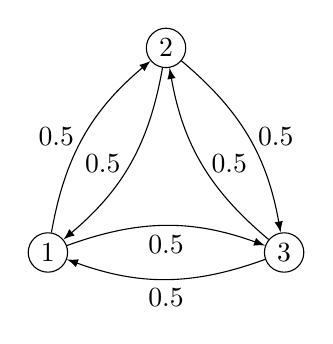
\begin{tikzpicture}[
        vertex/.style={circle, draw, minimum size=0.5cm, inner sep=0pt},
        baseline=(current bounding box.center),
    ]
        \node[vertex] (1) at (0, 0) {$1$};
        \node[vertex] (2) at (1.5, {1.5 * sqrt(3)}) {$2$};
        \node[vertex] (3) at (3, 0) {$3$}; 

        \draw[-latex] (1) to[bend left=20] node[left] {$0.5$} (2);
        \draw[-latex] (1) to[bend left=20] node[below] {$0.5$} (3);
        \draw[-latex] (2) to[bend left=20] node[left] {$0.5$} (1);
        \draw[-latex] (2) to[bend left=20] node[right] {$0.5$} (3);
        \draw[-latex] (3) to[bend left=20] node[below] {$0.5$} (1);
        \draw[-latex] (3) to[bend left=20] node[right] {$0.5$} (2);
    \end{tikzpicture}
\end{minipage}%
\begin{minipage}[c]{0.5\textwidth}
    \begin{equation}
        \mathcal{P} =
        \begin{pmatrix}
             0  & 0.5 & 0.5 \\
            0.5 &  0  & 0.5 \\
            0.5 & 0.5 &  0
        \end{pmatrix}
    \end{equation}
\end{minipage}
\vfill
\noindent
\begin{minipage}[c]{0.5\textwidth}
    \centering
    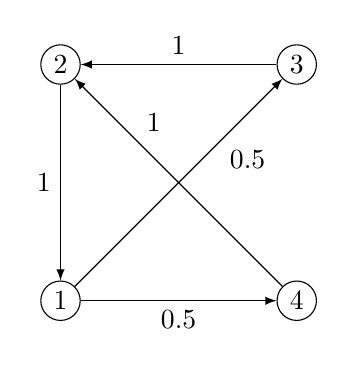
\begin{tikzpicture}[
        vertex/.style={circle, draw, minimum size=0.5cm, inner sep=0pt},
        baseline=(current bounding box.center),
    ]
        \node[vertex] (1) at (0, 0) {$1$};
        \node[vertex] (2) at (0, 3) {$2$};
        \node[vertex] (3) at (3, 3) {$3$};
        \node[vertex] (4) at (3, 0) {$4$};

        \draw[-latex] (1) to node[pos=0.7, below right] {$0.5$} (3);
        \draw[-latex] (1) to node[below] {$0.5$} (4);
        \draw[-latex] (2) to node[left] {$1$} (1);
        \draw[-latex] (3) to node[above] {$1$} (2);
        \draw[-latex] (4) to node[pos=0.7, above right] {$1$} (2);
    \end{tikzpicture}
\end{minipage}%
\begin{minipage}[c]{0.5\textwidth}
    \begin{equation}
        \mathcal{P} = 
        \begin{pmatrix}
            0 & 0 & 0.5 & 0.5 \\
            1 & 0 &  0  &  0  \\
            0 & 1 &  0  &  0  \\
            0 & 1 &  0  &  0
        \end{pmatrix}
    \end{equation}
\end{minipage}

\noindent
\begin{minipage}[c]{0.5\textwidth}
    \centering
    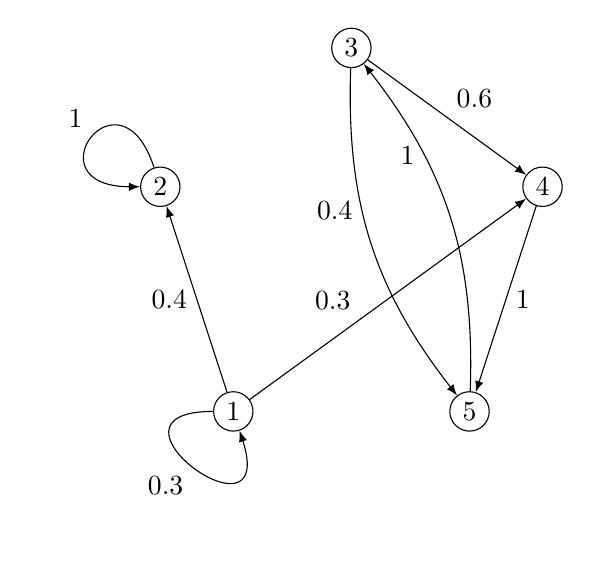
\begin{tikzpicture}[
        vertex/.style={circle, draw, minimum size=0.5cm, inner sep=0pt},
        baseline=(current bounding box.center),
    ]
        \def\radius{2.551952}
        \node[vertex] (1) at (234:\radius) {$1$};
        \node[vertex] (2) at (162:\radius) {$2$};
        \node[vertex] (3) at (90:\radius) {$3$};
        \node[vertex] (4) at (18:\radius) {$4$};
        \node[vertex] (5) at (306:\radius) {$5$};

        \draw[-latex] (1) to[out=180, in=288, looseness=10]
                          node[below left] {$0.3$} (1);
        \draw[-latex] (1) to node[left] {$0.4$} (2);
        \draw[-latex] (1) to node[pos=0.4, above left] {$0.3$} (4);
        \draw[-latex] (2) to[out=108, in=180, looseness=12]
                          node[above left] {$1$} (2);
        \draw[-latex] (3) to node[above right] {$0.6$} (4);
        \draw[-latex] (3) to[bend right=20] node[pos=0.4, left] {$0.4$} (5);
        \draw[-latex] (4) to node[right] {$1$} (5);
        \draw[-latex] (5) to[bend right=20] node[pos=0.7, left] {$1$} (3);
    \end{tikzpicture}
\end{minipage}%
\begin{minipage}[c]{0.5\textwidth}
    \begin{equation}
        \mathcal{P} =
        \begin{pmatrix}
            0.3 & 0.4 &  0  &  0  & 0.3 \\
             0  &  1  &  0  &  0  &  0  \\
             0  &  0  &  0  & 0.6 & 0.4 \\
             0  &  0  &  0  &  0  &  1  \\
             0  &  0  &  1  &  0  &  0
        \end{pmatrix}
    \end{equation}
\end{minipage}

For the third exercise, let’s consider the Markov chain defined by the matrix
\begin{equation}
    \mathcal{P}_{1} =
    \begin{pmatrix}
        1/2 & 1/2 \\
         1  &  0
    \end{pmatrix}.
\end{equation}
Is it irreducible? For every pair of states but one, $(2, 2)$, the corresponding
entry in $\mathcal{P}_1$ is different from zero. So, we can directly reach $1$
from $1$ and $2$, and $2$ from $1$. We have to find a path of any length $n$
that starts from $2$ and comes back to $2$, i.e. a $n$ such that $p^{n}_{ij} >
0$. Let’s see:
\begin{equation}
    \mathcal{P}_{1}^{2} =
    \begin{pmatrix}
        3/4 & 1/2 \\
        1/2 & 1/2
    \end{pmatrix}.
\end{equation}
So, there is a path of length $2$ that starts from $2$ and ends back there –
indeed, we can go from $2$ to $1$ with probability $1$ and then from $1$ to $2$
with probability $1/2$. Therefore, the Markov chain described by $\mathcal{P}_1$
is irreducible.

To find $\mathcal{P}_1^{n}$, it is best to diagonalize the matrix first:
\begin{equation}
    \mathcal{P}_{1}^{n} = T \mathcal{D}^{n} T^{-1}.
\end{equation}
The transformation matrix is given by
\begin{equation}
    T =
    \begin{pmatrix}
        1 & 1 \\
        1 & -2
    \end{pmatrix},
\end{equation}
while the diagonal matrix to the $n$-th power is
\begin{equation}
    \mathcal{D}^{n} =
    \begin{pmatrix}
        1 & 0 \\
        0 & -1/2
    \end{pmatrix}^n
    =
    \begin{pmatrix}
        1 & 0 \\
        0 & (-2)^{-n}
    \end{pmatrix}.
\end{equation}
Putting all together we obtain
\begin{equation}
    \mathcal{P}_{1}^{n} =
    \begin{pmatrix}
        1 & 1 \\
        1 & -2
    \end{pmatrix}
    \begin{pmatrix}
        1 & 0 \\
        0 & 2^{-n}
    \end{pmatrix}
    \begin{pmatrix}
        2/3 & 1/3 \\
        1/3 & -1/3
    \end{pmatrix}
    =\frac{1}{3}
    \begin{pmatrix}
        2 + (-1)^{n} 2^{-n} & 1 - (-1)^{n} 2^{-n} \\
        2 - (-1)^{n} 2^{1-n} & 1 + (-1)^{n} 2^{1-n}
    \end{pmatrix}.
\end{equation}
In the limit $n\to \infty$ this becomes
\begin{equation}
    \lim_{n \to \infty} \mathcal{P}_{1}^{n} =
    \begin{pmatrix}
        2/3 & 1/3 \\
        2/3 & 1/3
    \end{pmatrix}.
\end{equation}

Now, for the second matrix:
\begin{equation}
    \mathcal{P}_{2} =
    \begin{pmatrix}
         0  &  0  &  1  \\
         0  &  1  &  0  \\
        1/4 &  0  & 3/4
    \end{pmatrix},
\end{equation}
let’s find directly $\mathcal{P}_2^{n}$. The transformation matrix is
\begin{equation}
    T =
    \begin{pmatrix}
        -4 & 1 & 0 \\
        0 & 0 & 1 \\
        1 & 1 & 0
    \end{pmatrix},
\end{equation}
while the diagonalized one to the $n$-th power is
\begin{equation}
    \mathcal{D}^{n} =
    \begin{pmatrix}
        -1/4 & 0 & 0 \\
        0 & 1 & 0 \\
        0 & 0 & 1
    \end{pmatrix}^n
    =
    \begin{pmatrix}
        (-1)^{n} 4^{-n} & 0 & 0 \\
        0 & 1 & 0 \\
        0 & 0 & 1
    \end{pmatrix}.
\end{equation}
Putting everything together,
\begin{equation}
\begin{split}
    \mathcal{P}_2^{n} &=
    \begin{pmatrix}
        -4 & 1 & 0 \\
        0 & 0 & 1 \\
        1 & 1 & 0
    \end{pmatrix}
    \begin{pmatrix}
        (-1)^{n} 4^{-n} & 0 & 0 \\
        0 & 1 & 0 \\
        0 & 0 & 1
    \end{pmatrix}
    \begin{pmatrix}
        -1/5 & 0 & 1/5 \\
        1/5 & 0 & 4/5 \\
        0 & 1 & 0
    \end{pmatrix} \\
                      &= \frac{1}{5}
    \begin{pmatrix}
        1 + (-1)^{n} 4^{1-n} & 0 & 4 - (-1)^{n} 4^{1-n} \\
        0 & 5 & 0 \\
        1 - (-1)^{n} 4^{-n} & 0 & 4 + (-1)^{n} 4^{-n}
    \end{pmatrix}.
\end{split}
\end{equation}
Therefore, since $\mathcal{P}_{2}^{n}$ has entries which are zero, the
corresponding chain is \emph{not} irreducible. The limit $n \to \infty$ is
\begin{equation}
    \lim_{n \to \infty} \mathcal{P}_{2}^{n} =
    \begin{pmatrix}
        1/5 & 0 & 4/5 \\
        0 & 1 & 0 \\
        1/5 & 0 & 4/5
    \end{pmatrix}.
\end{equation}

Moving to the next exercise, the goal is to prove whether a Markov chain defined
by a given matrix is regular. To do it, it suffices to find a $n$ such that
every entry of $\mathcal{P}^{n}$ is positive. This implies that every entry of
$\mathcal{P}^{m}$ is positive whenever $m \geq n$. In the first case it is
simple, $n = 2$ suffices to end the proof:
\begin{equation}
    \begin{pmatrix}
        1/2 & 1/4 & 1/4 \\
        1/2 &  0  & 1/2 \\
        1/4 & 1/4 & 1/2
    \end{pmatrix}^2
    = \frac{1}{16}
    \begin{pmatrix}
        7 & 3 & 6 \\
        6 & 4 & 6 \\
        6 & 3 & 7
    \end{pmatrix}.
\end{equation}

The second matrix instead is problematic:
\begin{equation}
    \begin{pmatrix}
        1 & 0 \\
        1/2 & 1/2
    \end{pmatrix}.
\end{equation}
If we look at it, we can realize that we cannot reach state $2$ from state $1$
in any way. So, the associated chain is reducible and irregular.

In the following exercise, the stochastic matrix is
\begin{equation}
    \mathcal{P} =
    \begin{pmatrix}
        p  & 1-p &  0  &  0  \\
        0  &  0  &  p  & 1-p \\
        p  & 1-p &  0  &  0  \\
        0  &  0  &  p  & 1-p
    \end{pmatrix}.
\end{equation}
Let’s try to skip the calculations this time. If we consider state $1$, from the
first row we see that we can reach $2$ directly; from $2$ we can then reach $3$
and $4$. From $2$ we can reach $3$ and $4$; to reach $1$ we can pass through
$3$, since $p_{31} \neq 0$. $3$ and $4$ present the same situation as $1$ and
$2$ respectively. We can thus conclude that the associated Markov chain is
recurrent irreducible.

As for periodicity, if we square the matrix we get
\begin{equation}
    \mathcal{P}^{2} =
    \begin{pmatrix}
        p^{2} & p(1-p) & p(1-p) & (1-p)^{2} \\
        p^{2} & p(1-p) & p(1-p) & (1-p)^{2} \\
        p^{2} & p(1-p) & p(1-p) & (1-p)^{2} \\
        p^{2} & p(1-p) & p(1-p) & (1-p)^{2}
    \end{pmatrix},
\end{equation}
and this stays the same for all subsequent powers:
\begin{equation}
    \mathcal{P}^{3} =
    \begin{pmatrix}
        p^{2} & p(1-p) & p(1-p) & (1-p)^{2} \\
        p^{2} & p(1-p) & p(1-p) & (1-p)^{2} \\
        p^{2} & p(1-p) & p(1-p) & (1-p)^{2} \\
        p^{2} & p(1-p) & p(1-p) & (1-p)^{2}
    \end{pmatrix},
\end{equation}
and so on. So, the chain is definitely aperiodic, since all the entries of
$\mathcal{P}^{n}$ for $n > 1$ are positive.

To find the fixed point, we have to solve for $\pi$ the equation
\begin{equation}
    \pi \mathcal{P} = \pi \iff \mathcal{P}\tran \pi\tran = \pi\tran
    \iff (\mathcal{P}\tran - \I) \pi\tran = 0.
\end{equation}
This leads to the system of equations
\begin{equation}
    \begin{cases}
        (p-1)\pi_1 + \pi_3 = 0, \\
        (1-p)\pi_1 - \pi_2 +(1-p)\pi_3 = 0, \\
        p\pi_2 - \pi_3 + \pi_4 = 0, \\
        (1-p)\pi_2 - p\pi_4 = 0.
    \end{cases}
    \implies \dots \implies
    \begin{dcases}
        \pi_1 = \frac{p^{2}}{(1-p)^{2}}\pi_4, \\
        \pi_2 = \frac{p}{1-p}\pi_4, \\
        \pi_3 = \frac{p}{1-p}\pi_4.
    \end{dcases}
\end{equation}
Therefore, given a $q \in [0,1]$, the corresponding stationary $\pi$ is
\begin{equation}
    \pi_{q} = \left(\frac{p^{2}q}{(1-p)^{2}}, \frac{pq}{1-p}, \frac{pq}{1-p},
    q\right)
\end{equation}

The last exercise asked to find another stationary distribution. The matrix is
\begin{equation}
    \mathcal{P} =
    \begin{pmatrix}
        1/2 & 1/2 &  0  \\
        1/4 & 1/2 & 1/4 \\
         0  & 1/2 & 1/2
    \end{pmatrix}.
\end{equation}
The system corresponding to the equation $(\mathcal{P}\tran - \I) \pi\tran = 0$
is then
\begin{equation}
    \begin{pmatrix}
        -1/2 & 1/4 & 0 \\
        1/2 & -1/2 & 1/2 \\
        0 & 1/4 & -1/2
    \end{pmatrix}
    \begin{pmatrix}
        \pi_1 \\ \pi_2 \\ \pi_3 \\
    \end{pmatrix}
    =
    \begin{pmatrix}
        0 \\ 0 \\ 0
    \end{pmatrix}
    \implies
    \begin{cases}
        \pi_1 = \pi_3, \\
        \pi_2 = 2\pi_3.
    \end{cases}
\end{equation}
The stationary distribution is then given by the state vectors
\begin{equation}
    \pi_q = (q, 2q, q) \quad\text{with } q \in [0, 1].
\end{equation}
